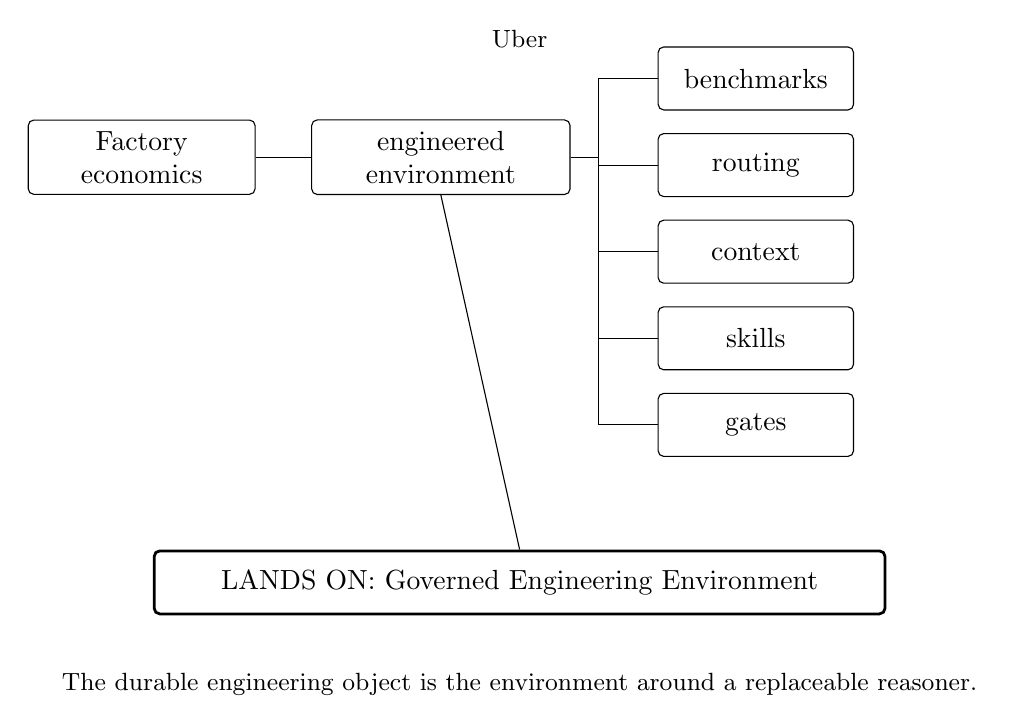
\begin{tikzpicture}[x=1cm,y=1cm,font=\magefigurefont\fontsize{10}{12}\selectfont,
box/.style={draw=black,fill=white,rounded corners=2pt,align=center,text width=3cm,minimum height=8mm,inner sep=4pt},
gate/.style={box,line width=1pt},note/.style={align=center,fill=white,inner sep=1pt,font=\magefigurefont\fontsize{9}{11}\selectfont},
edge/.style={-{Stealth[length=2mm]},line width=.6pt},optional/.style={edge,dashed},
every node/.style={text=black,execute at begin node={\hyphenpenalty=10000\exhyphenpenalty=10000}}]
\node[note,text width=12cm] (t5) at (0,1.5) {Uber};
\node[box,text width=2.6cm] (entry) at (-4.8,0) {Factory economics};
\node[box,text width=3cm] (hub) at (-1,0) {engineered environment};
\draw[draw] (entry) -- (hub);
\node[box,text width=2.2cm] (p0) at (3,1.0) {benchmarks};
\draw (hub.east) -- ++(.35,0) |- (p0.west);
\node[box,text width=2.2cm] (p1) at (3,-0.10000000000000009) {routing};
\draw (hub.east) -- ++(.35,0) |- (p1.west);
\node[box,text width=2.2cm] (p2) at (3,-1.2000000000000002) {context};
\draw (hub.east) -- ++(.35,0) |- (p2.west);
\node[box,text width=2.2cm] (p3) at (3,-2.3000000000000003) {skills};
\draw (hub.east) -- ++(.35,0) |- (p3.west);
\node[box,text width=2.2cm] (p4) at (3,-3.4000000000000004) {gates};
\draw (hub.east) -- ++(.35,0) |- (p4.west);
\node[gate,text width=9cm] (land) at (0,-5.4) {LANDS ON: Governed Engineering Environment};
\node[note,text width=12cm] (t20) at (0,-6.7) {The durable engineering object is the environment around a replaceable reasoner.};
\draw (hub.south)--(land.north);
\end{tikzpicture}
